% Chapter 6 — GPU Architecture, CUDA Programming, and Maximizing Occupancy  (v2: narrative edition)
% 53 pages; Part I follows the BOOK section order (SM internals -> threads/warps/blocks/grids -> limits -> PTX);
% 4 presenter intuition pages at 7, 9, 14, 15. Page numbers differ from v1. Use chapter06-lecture-script-v2-zh.md.
% v2 changes: book-plan opening (p2: SIMT -> CUDA -> memory -> roofline), question-driven roadmap (p3), worked-example p14, takeaway titles,
% unified workshop metaphor, occupancy caveat at p16, part-transition bridges, Plain-English takeaway bars.
% Compile: pdflatex chapter06-presentation-v2.tex  (run twice)
\documentclass[aspectratio=169]{beamer}

% ====== Presenter info: EDIT ME ======
\newcommand{\PresenterName}{Tianqin Cai}          % <-- 改成你的名字
\newcommand{\PresenterTitle}{Applied Scientist} % <-- 改成你的头衔
\newcommand{\PresenterOrg}{AWS}
% =====================================

\usetheme{Madrid}
\definecolor{navy}{RGB}{18,47,90}
\definecolor{kwblue}{RGB}{0,56,132}
\definecolor{okgreen}{RGB}{80,130,20}
\usecolortheme[named=navy]{structure}
\setbeamercolor{frametitle}{bg=navy,fg=white}
\setbeamercolor{title}{bg=navy,fg=white}
\setbeamercolor{block title}{bg=navy,fg=white}
\setbeamercolor{block body}{bg=gray!12,fg=black}
\setbeamercolor{block title example}{bg=okgreen,fg=white}
\setbeamercolor{block body example}{bg=okgreen!10,fg=black}
\setbeamertemplate{navigation symbols}{}
\setbeamertemplate{blocks}[rounded][shadow=true]

\usepackage{booktabs}
\usepackage{listings}
\lstset{
  language=C++,
  basicstyle=\ttfamily\fontsize{6.5}{7.6}\selectfont,
  keywordstyle=\color{kwblue}\bfseries,
  commentstyle=\color{gray}\itshape,
  stringstyle=\color{okgreen},
  showstringspaces=false,
  breaklines=true,
  columns=fullflexible
}

\newcommand{\kw}[1]{\textbf{\textcolor{kwblue}{#1}}}
\newcommand{\pe}[1]{\par{\setlength{\fboxsep}{2.5pt}\noindent\colorbox{navy!9}{\parbox{\dimexpr\textwidth-5pt\relax}{\footnotesize\itshape Plain English: #1}}}}
\newcommand{\bridge}[1]{{\footnotesize\itshape\textcolor{gray}{#1}}\par}
\newcommand{\refmark}[1]{\textsuperscript{[#1]}}

\title[AI Systems Performance Engineering]{AI Systems Performance Engineering}
\subtitle{Chapter 6 --- GPU Architecture, CUDA Programming, and Maximizing Occupancy\\{\small Part III structure preview (draft)}}
\author[\PresenterName\ \ \PresenterTitle\ \ \PresenterOrg]{\PresenterName\\\PresenterTitle\\\PresenterOrg}
\institute[]{\footnotesize Internal Training for Applied Scientists on AI Infrastructure}
\date{August 15, 2026}

\begin{document}

% ================================================================ 1
\begin{frame}
  \titlepage
\end{frame}

% ================================================================ 2
\begin{frame}{Part III --- The Memory Ladder at a Glance}
  \bridge{We can now create plenty of threads --- but what are they all waiting for? Usually data.}
  \begin{columns}[c]
    \column{0.58\textwidth}
    {\scriptsize\setlength{\tabcolsep}{3.5pt}
    \begin{tabular}{@{}lllll@{}}
      \toprule
      \textbf{Level} & \textbf{Scope} & \textbf{Capacity} & \textbf{Latency} & \textbf{BW} \\
      \midrule
      Registers & thread & 256 KB / SM & $\sim$1 cyc & 10s TB/s \\
      Shared + L1 & SM & 228 KB usable & 20--30 cyc & TB/s \\
      TMEM & SM & 256 KB (TC) & $\sim$10 cyc & TB/s \\
      Const cache & SM & 8 of 64 KB & 1 cyc bcast & TB/s \\
      L2 cache & GPU & \kw{126 MB} & $\sim$200 cyc & multi-TB/s \\
      Local (spill) & thread & DRAM-backed & $\leq$1000 cyc & --- \\
      Global HBM3e & device & \kw{180 GB} (B200) & $\leq$1000 cyc & \kw{$\sim$8 TB/s} \\
      \bottomrule
    \end{tabular}}\\[4pt]
    {\scriptsize Table 6-5. Every level trades capacity for latency/bandwidth.}
    \column{0.39\textwidth}
    \centering
    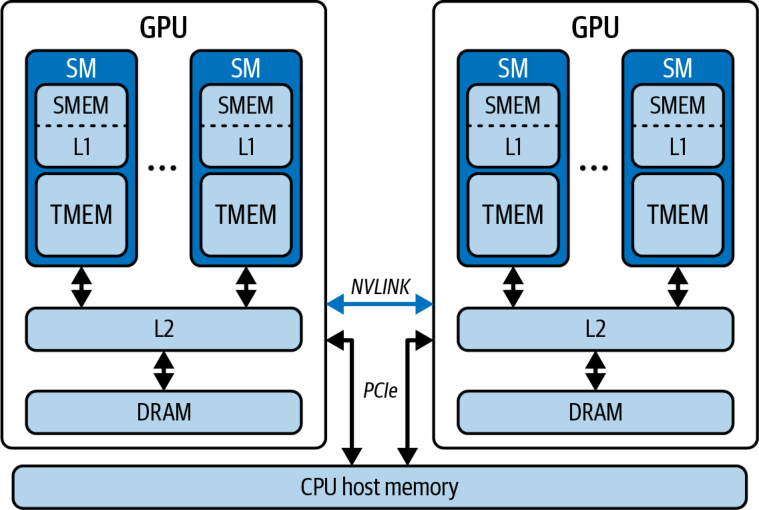
\includegraphics[width=\linewidth]{figs/fig6-10.png}\\
    {\scriptsize Figure 6-10. GPU memory hierarchy, including the CPU}
  \end{columns}
  \pe{your \kw{own toolbox} (registers) $\to$ the \kw{shared workbench} (shared) $\to$ the factory's \kw{central depot} (L2) $\to$ the \kw{distant warehouse} (HBM) --- do the work at your bench.}
\end{frame}

% ================================================================ 3
\begin{frame}{Register Pressure Can Turn Fast Storage into DRAM Access}
  \begin{columns}[c]
    \column{0.55\textwidth}
    \begin{itemize}
      \item Every thread ``begins its journey'' at the \kw{register file}: single-cycle reads/writes,
            contending with almost nothing --- \kw{tens of TB/s per SM}.
      \item Budget: 64K registers per SM, \kw{max 255 per thread}.
      \item The cliff: need more (too many locals, compiler temporaries) $\Rightarrow$
            overflow \kw{spills into local memory} --- which despite the name lives in
            \kw{off-chip DRAM}: hundreds to 1000+ cycles.
      \item Watch \kw{``Registers Per Thread''} in Nsight Compute --- spills are silent killers.
    \end{itemize}
    \column{0.42\textwidth}
    \centering
    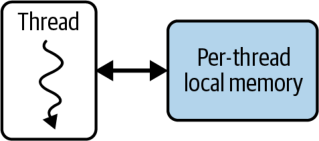
\includegraphics[width=0.6\linewidth]{figs/fig6-12.png}\\
    {\scriptsize Figure 6-12. Per-thread local memory (spill space, DRAM-backed)}
  \end{columns}
  \pe{``local memory'' is a self-storage unit across town, not your pocket.}
\end{frame}

% ================================================================ 4
\begin{frame}[fragile]{Shared Memory + L1: One SRAM, Two Jobs}
  \begin{columns}[c]
    \column{0.55\textwidth}
    \begin{itemize}
      \item One \kw{256 KB SRAM per SM}, split between user-managed \kw{shared memory}
            (up to 228 KB; 227 usable per block) and \kw{L1/data cache}.
      \item You choose the \kw{carveout}:
    \end{itemize}
\begin{lstlisting}
cudaFuncSetAttribute(myKernel,
  cudaFuncAttributePreferredSharedMemoryCarveout,
  carveoutPercent);
\end{lstlisting}
    \begin{itemize}
      \item $\sim$20--30 cycles; \kw{TB/s} if you avoid \kw{bank conflicts}
            (multiple threads hitting the same memory bank $\Rightarrow$ serialized access).
      \item This is the workbench for \kw{intrablock cooperation} --- tiles, reductions, staging.
    \end{itemize}
    \column{0.42\textwidth}
    \centering
    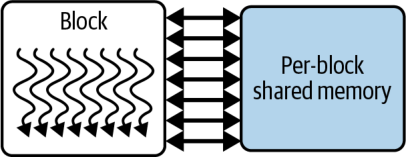
\includegraphics[width=0.75\linewidth]{figs/fig6-13.png}\\
    {\scriptsize Figure 6-13. Thread-block shared memory}
  \end{columns}
  \pe{one workbench, adjustable split: how much is your team's project table vs.\ the automatic cache shelf.}
\end{frame}

% ================================================================ 5
\begin{frame}{TMEM and TMA: Feeding the Tensor Cores}
  \begin{columns}[c]
    \column{0.55\textwidth}
    \begin{itemize}
      \item \kw{TMEM}: dedicated \kw{256 KB per-SM SRAM}, the \kw{accumulator} for 5th-gen
            Tensor Core ops (\texttt{tcgen05.*}, \kw{UMMA}); talks to Tensor Cores at tens of TB/s.
      \item \kw{Not pointer-addressable} from CUDA C++ --- data movement is orchestrated by the
            \kw{TMA} (Tensor Memory Accelerator) via \kw{descriptors}.
      \item For $C = A \times B$: operand B in SMEM, A + accumulator in TMEM; TMA moves tiles
            HBM $\to$ L2 $\to$ SMEM; SMEM $\leftrightarrow$ TMEM implicit via Tensor Core ops.
      \item Net effect: \kw{reduces Tensor Core reliance on global memory}. Details: Chapter 10.
    \end{itemize}
    \column{0.42\textwidth}
    \centering
    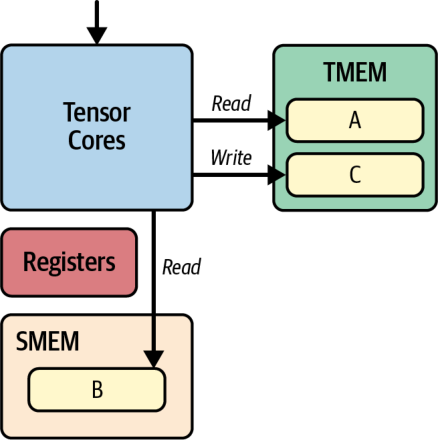
\includegraphics[width=0.72\linewidth]{figs/fig6-11.png}\\
    {\scriptsize Figure 6-11. TMEM + SMEM servicing Tensor Cores for $C = A\times B$}
  \end{columns}
  \pe{TMA is a forklift crew moving pallets in the background; the chefs never leave the kitchen.}
\end{frame}

% ================================================================ 6
\begin{frame}{Constant Cache: One-Cycle Broadcast}
  \begin{columns}[t]
    \column{0.52\textwidth}
    \begin{itemize}
      \item $\sim$\kw{8 KB cache per SM} fronting the 64 KB \kw{\texttt{\_\_constant\_\_}} space.
      \item Superpower: when all 32 threads of a warp load \kw{the same address},
            the cache \kw{broadcasts} the value in a \kw{single cycle} --- as fast as a register.
      \item Divergent reads \kw{serialize across lanes}; misses cost more --- so it's for
            \kw{small, read-only, uniformly-accessed} data.
    \end{itemize}
    \column{0.45\textwidth}
    \begin{exampleblock}{The book's LLM examples}
      \begin{itemize}\small
        \item Rotary positional encoding (RoPE) lookup tables
        \item ALiBi slopes
        \item LayerNorm $\gamma$/$\beta$ vectors
        \item Embedding quantization scales
      \end{itemize}
      \smallskip
      {\small Shared by every thread with \kw{zero global-memory traffic}.}
    \end{exampleblock}
  \end{columns}
  \pe{a megaphone, not a mailbox: one announcement reaches all 32 workers at once --- but only if they all asked the same question.}
\end{frame}

% ================================================================ 7
\begin{frame}{L2 Cache: The GPU-Wide Middleman}
  \begin{columns}[t]
    \column{0.52\textwidth}
    \begin{itemize}
      \item \kw{126 MB} shared by all SMs --- the glue between on-chip SRAM and off-chip HBM3e.
      \item $\sim$200 cycles, aggregate bandwidth in the \kw{tens of TB/s}; absorbs L1 spillover.
      \item \kw{Cross-block reuse}: data fetched by one thread block is reused by others
            \kw{without revisiting DRAM}.
    \end{itemize}
    \column{0.45\textwidth}
    \begin{block}{The coalescing rule (book tip)}
      \small Structure global loads into \kw{128-byte aligned, coalesced} segments that map
      cleanly to cache lines --- avoids split transactions, maximizes L2 \kw{and} DRAM
      bandwidth. (How-to: Chapter 7.)
    \end{block}
  \end{columns}
  \pe{L2 is the factory's \kw{central depot}: if another crew already fetched the part from the warehouse, you grab it here --- provided everyone orders \kw{whole pallets}, not single screws.}
\end{frame}

% ================================================================ 8
\begin{frame}{Global HBM3e, the Dual-Die B200, and Coherency}
  \begin{columns}[c]
    \column{0.55\textwidth}
    \begin{itemize}
      \item \kw{180 GB} on B200 ($\sim$288 GB on B300) at \kw{$\sim$8 TB/s} --- but
            \kw{hundreds to 1000+ cycles}: the slowest link in the chain.
      \item Register spills and oversized automatic arrays (local memory) also pay this price.
      \item \kw{Fun fact (book note)}: B200 = \kw{two reticle-limited dies} joined by a
            \kw{10 TB/s} chip-to-chip interconnect, 4 HBM3e stacks each ---
            presented to you as \kw{one GPU, one address space}.
      \item \kw{Point of coherency} (Figure 6-15): memory consistency is established at
            thread $\to$ block $\to$ cluster $\to$ device $\to$ system scope ---
            the wider the communication, the higher the cost.
    \end{itemize}
    \column{0.42\textwidth}
    \centering
    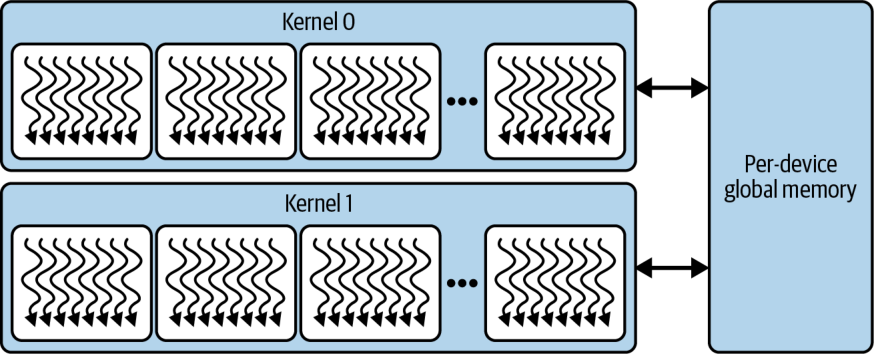
\includegraphics[width=\linewidth]{figs/fig6-14.png}\\[2pt]
    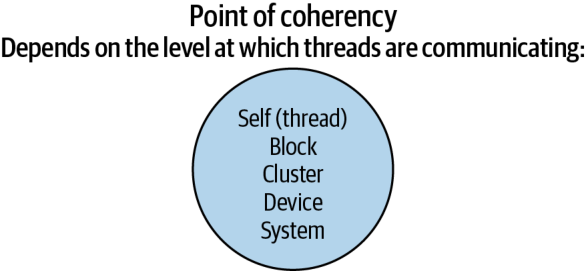
\includegraphics[width=0.9\linewidth]{figs/fig6-15.png}\\
    {\scriptsize Figures 6-14 / 6-15. Global memory; points of coherency}
  \end{columns}
\end{frame}

% ================================================================ 9
\begin{frame}{Unified Memory Hides Copies, Not Their Cost}
  \begin{columns}[c]
    \column{0.55\textwidth}
    \begin{itemize}
      \item \kw{\texttt{cudaMallocManaged()}}: one coherent CPU+GPU address space ---
            no separate buffers, no manual \texttt{cudaMemcpy}.
      \item Under the hood: pages \kw{migrate on demand} over whatever link connects CPU and GPU.
      \item The catch: a GPU touch of a CPU-resident page \kw{page-faults and stalls the kernel}.
      \item On PCIe: on-fault transfers can be \kw{slower than manual memcpy}.
            On Grace superchips, \kw{NVLink-C2C} ($\sim$900 GB/s) makes migrations near
            device-native --- \kw{but latency is never zero}.
    \end{itemize}
    \column{0.42\textwidth}
    \centering
    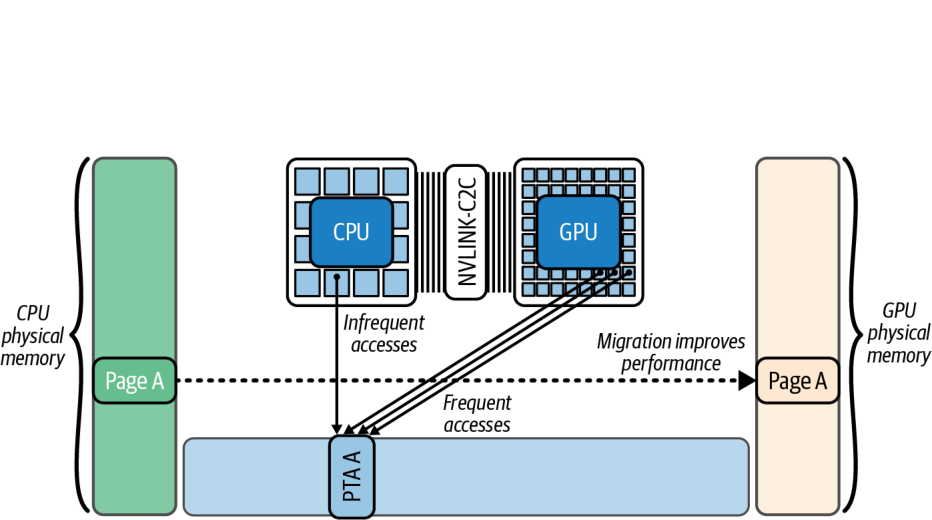
\includegraphics[width=\linewidth]{figs/fig6-16.png}\\
    {\scriptsize Figure 6-16. Automatic page migration with Unified Memory}
  \end{columns}
  \pe{Unified Memory is \kw{automatic parts delivery}: convenient --- but if the part isn't in the workshop when the crew needs it, \kw{the crew stands and waits}.}
\end{frame}

% ================================================================ 10
\begin{frame}[fragile]{Taming Unified Memory: Prefetch, Advise, Attach}
  \begin{columns}[t]
    \column{0.55\textwidth}
\begin{lstlisting}
// 1) move data BEFORE the kernel needs it:
cudaMemPrefetchAsync(ptr, size, gpuId, s);
// 2) tell the driver how you'll use it:
cudaMemAdvise(ptr, size,
    cudaMemAdviseSetPreferredLocation, gpuId);
cudaMemAdvise(ptr, size,
    cudaMemAdviseSetReadMostly, gpuId);
cudaMemAdvise(ptr, size,
    cudaMemAdviseSetAccessedBy, otherGpuId);
// 3) confine faults/migrations to one stream:
cudaStreamAttachMemAsync(stream, ptr, 0,
    cudaMemAttachSingle);
\end{lstlisting}
    \column{0.42\textwidth}
    \begin{itemize}\small
      \item \kw{Prefetch} turns first-touch migrations into \kw{overlappable async transfers}
            (Figure 6-17).
      \item \kw{ReadMostly} allows replicated read-only copies; \kw{AccessedBy} lets a second GPU
            map pages \kw{without} migration (Figure 6-18).
      \item \kw{Attach} stops \emph{other} streams from stalling on this range.
      \item No NVLink-C2C? Pin data \kw{NUMA-local} (peer copy / prefetch).
      \item Result: performance \kw{close to manual \texttt{cudaMemcpy}}, simplicity retained.
    \end{itemize}
  \end{columns}
\end{frame}

\end{document}
